\chapter[Analysis]{Analysis}

\section{Overview}
While Figure \ref{fig:alldata-GOES6-1983-1991} shows an overview of the most pertinent variables used in this study, some further analysis was done to determine any potential biases introduced by specifics of the satellite motion or derivations used. For example, Figure \ref{fig:ByHourExample} shows that not only did data availability vary significantly with magnetic local time (MLT), but the values themselves vary significantly. \vinote{Cite that this is known (dawn vs dusk, etc)}

\begin{figure}
\centering
\includegraphics[width=0.7\linewidth]{Figures/rhoMLT.eps}
\includegraphics[width=0.7\linewidth]{Figures/nansbyhour.eps}
\caption{Median \req\ binned by local time, and availability of \req\ with local time. \vinote{Ticks every 2 hours}}
\label{fig:ByHourExample}
\end{figure}

\section{$F_{10.7}$ Dependence}
\cite{Takahashi2010SolarCycleVariation} showed a strong correlation between the 27-day averaged $F_{10.7}$ index of solar activity and the averaged equatorial mass density (\req). This was chosen as a starting place for verifying the data analysis routines developed for this dataset, so as to show that data input, averaging, and interpolation were all done in a reasonable and reproducible manner. Figure \ref{fig:F107rhoeq27dcomparison} shows the strong correlation seen previously, and reasonably reproduces Figure 13.b from \cite{Takahashi2010SolarCycleVariation} for the years covered by GOES 6.

\begin{figure}
\centering
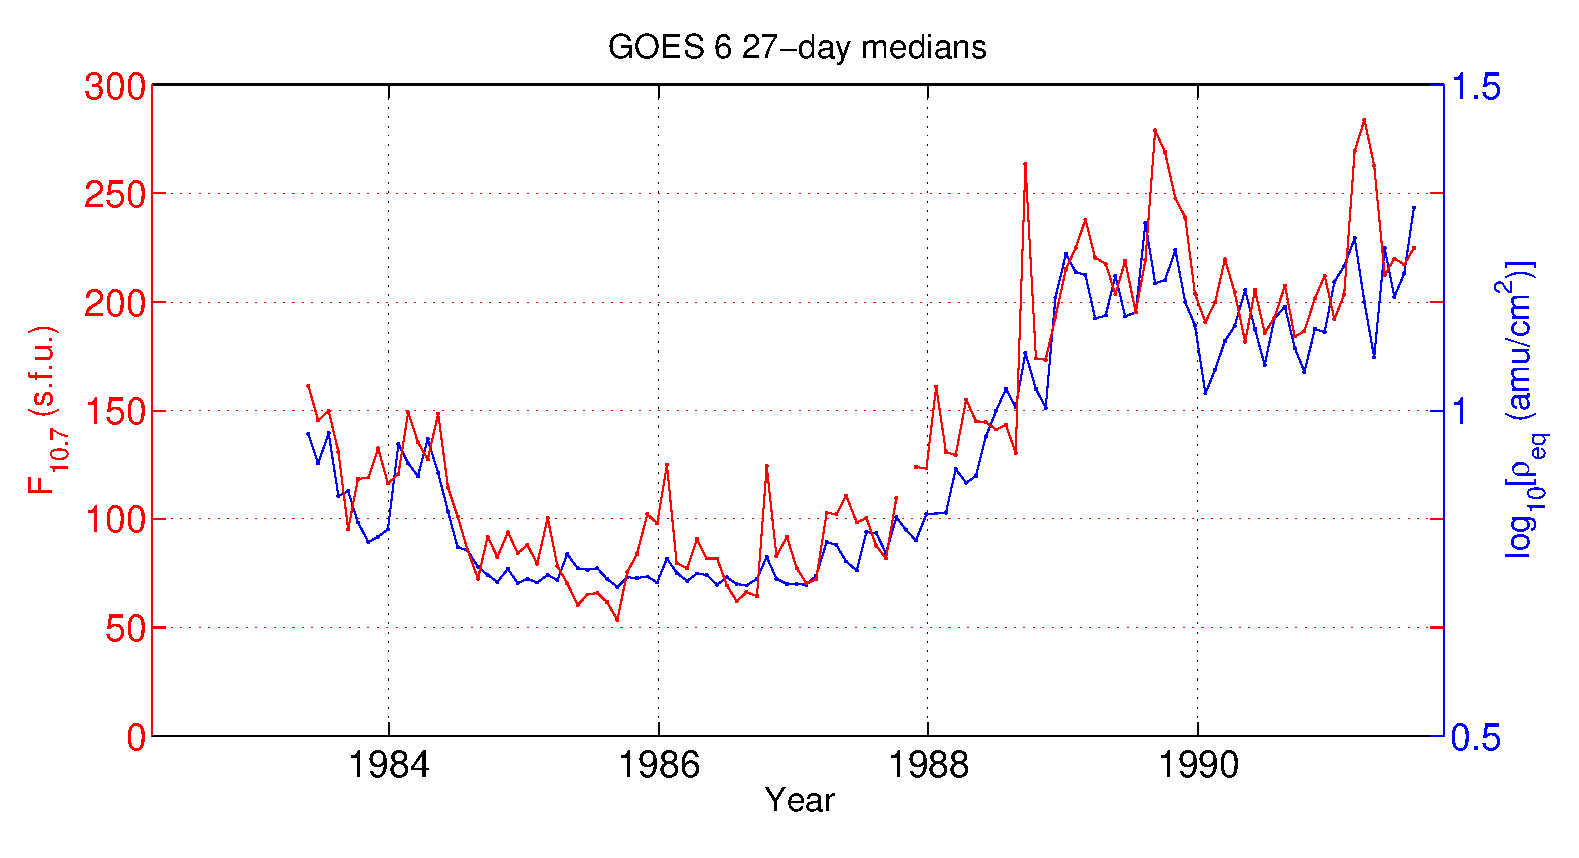
\includegraphics[width=0.7\linewidth]{Figures/F107MD27d-GOES6}
\caption{Comparing $F_{10.7\_27d}$ and $log(\rho_{eq\_27d})$ using GOES 6 data \vinote{Add all satellites with coverage}}
\label{fig:F107rhoeq27dcomparison}
\end{figure}

\section{Linear Correlations}
This dependence was further investigated, and extended, by creating a simple linear model for each major variable in the database as well as combinations of some to investigate independent contributions to the total correlation (by testing how much correlation improved in a combined model over either of the constituent models.)  The inputs were the median values of each variable for four hours before a \dst\ event onset, and they were trained to predict a median of the value at onset with the four hours following it. The models were trained on half of the dataset and tested on the other half for each satellite, and this was repeated with new random samples 100 times and then the median correlation values were taken. The results are shown in Table \ref{CCperltable}.

\begin{table}[h]
	\footnotesize
	\begin{tabular}{|L|LLLL|}
		\hline
		& \text{GOES 2} & \text{GOES 5} & \text{GOES 6} & \text{GOES 7}\\ \hline
		DoY & -0.07 & +0.14 & -0.04 & +0.06 \\
		MLT & -0.07 & -0.05 & -0.02 & -0.05 \\
		B_z & +0.19 & -0.13 & +0.09 & -0.09 \\
		V_{sw} & -0.04 & +0.27 & +0.05 & -0.05 \\
		D_{st} & +0.26 & +0.67 & +0.09 & +0.21 \\
		\rho_{sw} & +0.33 & +0.63 & +0.10 & +0.35 \\
		F_{10.7} & +0.42 & +0.16 & +0.51 & +0.42 \\
		B_z+V_{sw} & +0.10 & +0.18 & +0.11 & -0.12 \\
		D_{st}\text{+}F_{10.7} & +0.44 & +0.69 & +0.54 & +0.47 \\
		All & -0.06 & +0.34 & +0.62 & +0.40 \\
		\hline
	\end{tabular}
	\caption{Table of linear model correlations showing the median of 100 random samples. Each sample trained on half of the data (via randomly selected rows of the least squares matrix) and tested on the other half} 
	\label{CCperltable}
\end{table}



\vnote Look at making tables and figures a git submodule

It can be seen that $F_{10.7}$ almost always correlates the best with \req, but that there is significant variance between data from different satellites. \vinote{Include training correlations? Make model a 12 hour model to smooth it out a bit?}

\section{Nonlinear Correlations}

Similarly for a neural net model with the same input and target structure as the linear model, but training on a randomly selected 70\% of the data, testing on another 15\%, and validating on the remaining 15\%, Table \ref{NNperltable} shows the resulting correlation values for the validation data set.

\begin{table}[h]
	\small
	\begin{tabular}{|L|LLLL|}
		\hline
		& \text{GOES 2} & \text{GOES 5} & \text{GOES 6} & \text{GOES 7}\\ \hline
		DoY & +0.07 & +0.36 & +0.36 & +0.10 \\
		MLT & +0.33 & +0.20 & +0.27 & +0.18 \\
		B_z & +0.19 & +0.15 & +0.20 & -0.00 \\
		V_{sw} & +0.28 & +0.39 & +0.13 & +0.10 \\
		D_{st} & +0.03 & +0.08 & +0.05 & +0.19 \\
		\rho_{sw} & +0.02 & +0.04 & +0.21 & +0.05 \\
		F_{10.7} & +0.26 & +0.46 & +0.52 & +0.36 \\
		B_z+V_{sw} & +0.09 & +0.24 & +0.20 & +0.04 \\
		D_{st}+F_{10.7} & +0.28 & +0.33 & +0.54 & +0.33 \\
		All & +0.17 & +0.56 & +0.57 & +0.19 \\
		\hline
	\end{tabular}
	\caption{Table of nonlinear model correlations showing the median of 100 random samples. Each sample trained on half of the data (via randomly selected rows of the least squares matrix) and tested on the other half} 
	\label{NNperltable}
\end{table}

It should be noted that nonlinear modeling is much more susceptible to overfitting than linear modeling \vinote{cite?} due to the higher order of fitting done on training and validation data, as well as the lack of a straight-forward optimal error-minimization method such as least squares regression \vinote{(non-unique solution, non-guaranteed convergence, etc)}. This is why some models, such as that including every possible variable, correlate worse than models of just a few parts. Where a linear model can minimize error by zeroing out variables without useful information, the neural net will try to incorporate the information anyway and end up overfitting \vinote{Too much explanation?}.

